\documentclass{article}
\usepackage{url}
\usepackage{fullpage}
\usepackage{boxedminipage}

\parskip=1.25ex plus 1ex minus 1.25ex

% \VignetteIndexEntry{Introduction to the oce package}
% \VignetteDepends{oce}
% \VignetteKeyword{oceanography}

\newcommand{\workedexercise}[2]{
	\vspace{1ex}
	\begin{boxedminipage}[c]{0.95\linewidth}
		{\textbf{Exercise #1}.\hspace{1em}#2}
	\end{boxedminipage}
	\vspace{1ex}
}
\newcommand{\workedanswer}[1]{
\goodbreak
\vskip 1.5ex plus 0.5ex minus 0.5ex
\noindent\textbf{Exercise #1.} 
}


\usepackage{/Library/Frameworks/R.framework/Resources/share/texmf/Sweave}
\begin{document}

\title{The OCE package}
\author{Dan E. Kelley}
\maketitle

%--------- adjust textmate window until this just fits ----------------------------------------

\begin{abstract}

The \verb@oce@ package makes it easy to read, summarize and plot data from a variety of
Oceanographic instruments, isolating the researcher from the quirky data formats that are
common in this field. It also provides functions for working with basic seawater properties
such as the equation of state, and with derived quantities such as the buoyancy frequency.
Although simple enough to be used in a teaching context, \verb@oce@ is powerful enough for a
research setting.  These things are illustrated here with practical examples.

\end{abstract}

\section{Introduction}

Oceanographers must deal with measurements made by a wide variety of instruments, a task that
is complicated by the delight instrument manufacturers seem to take in inventing new data
formats. The manufacturers often provide software for scanning the data files and producing
some standard plots, but this is of limited use to researchers who work with several instrument
types at the same time, and who need to carry the analysis beyond the first step.

The need to scan diverse data files was just one motivation for the creation of \verb@oce@. The
other aim was to provide a system in which oceanographic data could be analyzed easily in R.
This second goal influenced the design of the objects in \verb@oce@, each of which blends three
components: (a) the data itself, e.g. vectors of pressure, temperature, and salinity from a CTD
instrument, (b) metadata inferred from the data file's header, e.g. the location at which a CTD
cast was made, and (c) processing-stage metadata, e.g. a time-stamped log of changes made to
the object by \verb@oce@ functions. This approach, along with a policy of adding features
according to the priorities of practical research, should make \verb@oce@ a comfortable tool
today, and should keep it relevant as it grows to incorporate new features.

\section{Calculations of seawater properties}

The \verb@oce@ package provides many functions for dealing with seawater properties. Probably
the most used is \verb@sw.rho(S,t,p)@, which computes seawater density $\rho$ as a function of
salinity $S$ (PSU), in-situ temperature $t$ ($^\circ$C \dots\/ note the use of lower-case in
this and related functions, to avoid confusion with \verb@T@, an abbreviation used sometimes in
R programs) and pressure $p$ (decibar). The result is a number in the order of $1000$kg/m$^3$.
For many purposes, Oceanographers prefer to use the density anomaly $\sigma=\rho-1000$kg/m$^3$,
provided with \verb@sw.sigma(S,t,p)@, or its adiabatic cousin $\sigma_\theta$, provided with
\verb@sw.sigma.theta(S,t,p)@.

Note that the names of functions relating to seawater material properties start with
``\verb@sw.@''; future versions of \verb@oce@ may add similarly named functions for the
properties of air, sediment, organisms, etc.

\looseness=1
Most of the functions use the UNESCO formulations of seawater properties, but new formulations
may be added as they come into use in the literature.
A partial list of seawater functions is as follows:
\verb@sw.N2@ (buoyancy freqency),
\verb@sw.S.C.T.p@ (salinity $S$ from $C$, $T$ and $p$),
\verb@sw.S.T.rho@ ($S$ from $T$ and $\rho$),
\verb@sw.T.S.rho@ ($T$ from $S$ and $\rho$),
\verb@sw.T.freeze@ (freezing temperature),
\verb@sw.alpha@ (thermal expansion coefficient $\alpha=-\rho_0^{-1}\partial\rho/\partial T$),
\verb@sw.beta@ (haline compression coefficient $\beta=\rho_0^{-1}\partial\rho/\partial S$),
\verb@sw.alpha.over.beta@ ($\alpha/\beta$),
\verb@sw.conductivity@ (conductivity from $S$, $T$ and $p$), 
\verb@sw.depth@ (depth from $p$ and latitude), 
\verb@sw.lapse.rate@ (adiabatic lapse rate), 
\verb@sw.rho@ (density $\rho$ from $S$, $T$ and $p$), 
\verb@sw.sigma@ ($\rho-1000$\,kg/m$^3$), 
\verb@sw.sigma.t@ ($\sigma$ with $p$ set to zero and temperature unaltered),
\verb@sw.sigma.theta@ ($\sigma$ with $p$ set to zero and temperature altered adiabatically),
\verb@sw.sound.speed@ (speed of sound in m/s),
\verb@sw.specific.heat@ (specific heat in J/kg/$^\circ$C),
\verb@sw.spice@ (a quantity used in double-diffusive research),
\verb@sw.theta@ (potential temperature in $^\circ$C),
and
\verb@sw.viscosity@ (viscosity).
Details and examples are, of course, provided in the documentation of these functions.


\workedexercise{1}{(a) What is the density of a seawater parcel at pressure
$100$dbar, with salinity $34$PSU and temperature $10^\circ$C?
(b) What temperature would the parcel have if raised adiabatically to the surface?
(c) What density would it have if raised adiabatically to the surface?
(d) What density would it have if lowered about 100m, increasing the pressure to $200$dbar?}


\section{CTD data}
\subsection{Example with pre-trimmed data}

To get you started with CTD data, \verb@oce@ provides a sample data set that has been trimmed to just the downcast portion of the sampling.  (See the next section to learn how to do this trimming.).  The commands
\begin{Schunk}
\begin{Sinput}
> library(oce)
> data(ctd)
> plot(ctd)
\end{Sinput}
\end{Schunk}
produce Figure~\ref{fig:ctd}. You may also get a summary of the data with
\begin{Schunk}
\begin{Sinput}
> summary(ctd)
\end{Sinput}
\end{Schunk}

The object used to hold CTD data stores not just the data, but also the raw header sequence,
and whatever has been discovered about the dataset by parsing the header; use
\begin{Schunk}
\begin{Sinput}
> names(ctd)
\end{Sinput}
\end{Schunk}
to learn about these metadata, and use
\begin{Schunk}
\begin{Sinput}
> names(ctd$data)
\end{Sinput}
\end{Schunk}
to find out what sensors were attached to the instrument, thus providing data columns. It is
possible to plot the components individually, either by accessing the data directly (see the
WOCE section, below, for an example) or by using more specialized functions such as
\verb@plot.TS@ and \verb@plot.profile@.
\begin{figure}
\begin{center}
\setkeys{Gin}{width=.8\textwidth}
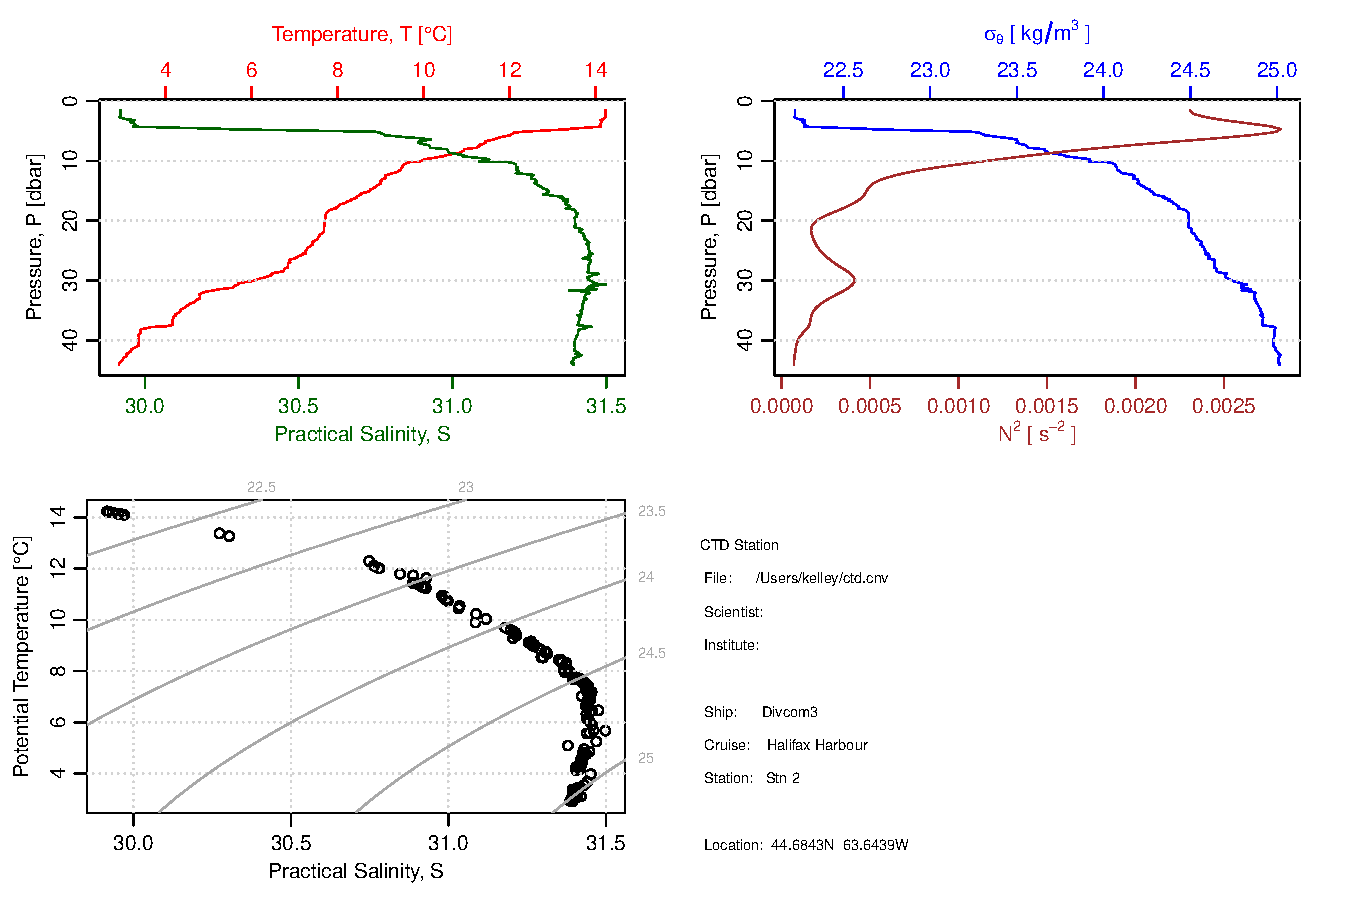
\includegraphics{oce-ctdfig}
\end{center}
\caption{Overview graph of the sample CTD dataset \texttt{ctd}, acquired during the St Lawrence Estuary Internal Wave Experiment.  (This dataset has been trimmed to just the downcast; see the text and Figure~\ref{fig:ctdraw} for more on trimming.)}
\label{fig:ctd}
\end{figure}

\workedexercise{2}{Plot a profile of $\sigma_\theta$ and $N^2$, for just the data in the pycnocline.}

\subsection{Example with raw data}

Practicing Oceanographers may be wondering how the CTD cast used in the preceding section was
trimmed of equilibration-phase and upcast-phase data. Data from these sections are spurious and
must be trimmed as a first step in processing. For example, consider the following code.
\begin{Schunk}
\begin{Sinput}
> data(ctd.raw)
> plot.ctd.scan(ctd.raw)
\end{Sinput}
\end{Schunk}
\begin{figure}
\begin{center}
\setkeys{Gin}{width=0.55\textwidth}
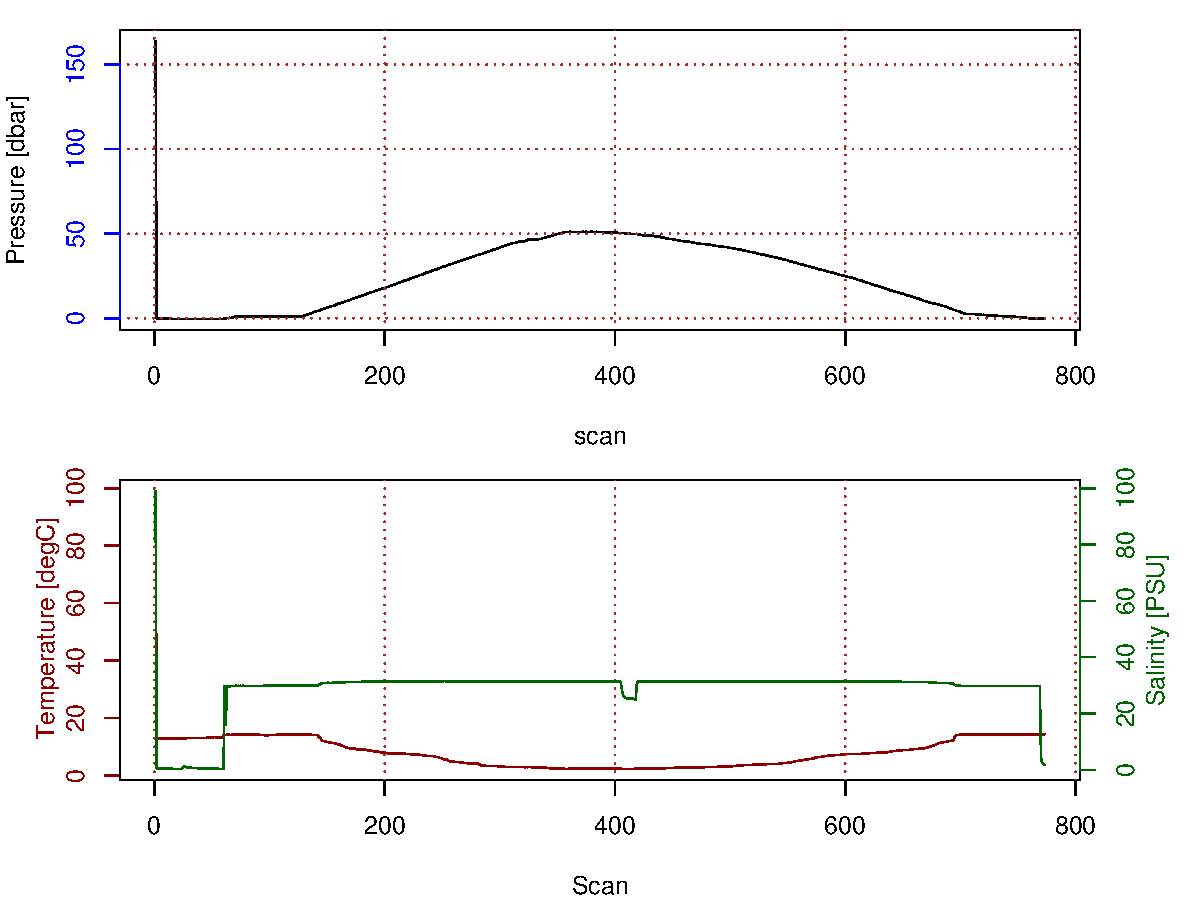
\includegraphics{oce-ctdrawfig}
\end{center}
\caption{Scanwise plot of the \texttt{ctd.raw} sample data set.  Note the wild spike at the start, the equilibration phase before the downcast, and the spurious freshening signal near the start of the upcast.  See the text for a discussion of how inspection of such graphs can help in trimming CTD data.}
\label{fig:ctdraw}
\end{figure}

\noindent This produces a two-panel plot (Figure~\ref{fig:ctdraw}) of the data as a
time-series, revealing not just the (useful) downcast, but also the subsequent upcast sequence.
The x-axis in this plot is the scan number, which is a convenient index for extraction of the
downcast portion of the profile by an essentially manual method, e.g. proceeding with a
sequence of commands such as
\begin{Schunk}
\begin{Sinput}
> plot.ctd.scan(ctd.trim(ctd.raw, "scan", c(140, 250)))
> plot.ctd.scan(ctd.trim(ctd.raw, "scan", c(150, 250)))
\end{Sinput}
\end{Schunk}
This is the ``gold standard'' method, which is recommended for detailed work. However, for
quick work, you may find that the automatic downcast detection scheme works adequately, e.g.
\begin{Schunk}
\begin{Sinput}
> ctd.trimmed <- ctd.trim(ctd.raw)
\end{Sinput}
\end{Schunk}

It should be noted that \verb@ctd.trim@ inserts entries into the object's log file, so that you
(or anyone else with whom you share the objec) will be able to track exactly how this trimming
was done.

Once the profile has been trimmed, you may wish to use \texttt{ctd.decimate()} to smooth the
data and interpolate the smoothed results to uniformly-spaced pressure values. For example, a
quick examination of a file might be done by the following:
\begin{Schunk}
\begin{Sinput}
> plot(ctd.decimate(ctd.trim(read.ctd("stn123.cnv"))))
\end{Sinput}
\end{Schunk}

\subsection{Example with WOCE archive data}

The package has a harder time scanning the headers of data files in the WOCE archive format than
it does in the Seabird format illustrated in the previous examples. This is mainly because
front-line researchers tend to work in the Seabird format, and partly because the WOCE format is
odd. For example, the first line of a WOCE file is of the form \texttt{CTD,20060609WHPOSIODAM}.
Only the first part of this is easy to scan. To the left of the comma is the string \texttt{CTD},
which seems straightforward, except that in some cases it is written \texttt{CTDO}. After the
comma is found the file date (yyyymmdd), and that is easy to parse. But then things get tricky.
The next sequence is a string of characters that indicate the division of the institute (WHPO),
the institute itself (SIO), and the name of the investigator (DAM). The problem is that no
dividers separate these items, and that there are no standards for the item lengths. The approach
to \verb@oce@ development is to tackle easy and important problemss before complicated special
cases, and so no attempt has been made to parse this part of the header. Of course, R provides
access to object constituents, so that a human working with this file could easily do e.g.
\begin{Schunk}
\begin{Sinput}
> x <- read.ctd("nnsa_00934_00001_ct1.csv", type = "WOCE")
> x$institute <- "SIO"
> x$scientist <- "DAM"
\end{Sinput}
\end{Schunk}

For a real-world example (with warts!), visit
\url{http://cchdo.ucsd.edu/data_access?ExpoCode=58JH199410} and download the zip file containing
the Arctic section called ``CARINA'', measured in 1994. Expand the zip file, enter the directory,
and run the code below. 
\begin{Schunk}
\begin{Sinput}
> library(oce)
> files <- system("ls *.csv", intern = TRUE)
> for (i in 1:length(files)) {
+     cat(files[i], "\n")
+     x <- read.ctd(files[i])
+     if (i == 1) {
+         plot.TS(x, xlim = c(31, 35.5), ylim = c(-1, 10), type = "l", 
+             col = "red")
+     }
+     else {
+         lines(x$data$salinity, x$data$temperature, col = "red")
+     }
+ }
\end{Sinput}
\end{Schunk}

What you'll see is an overall $T-S$ diagram for the entire dataset. It may take a while, since the
dataset contains over 90,000 observations. You may note that, even though this is an official,
quality-controlled dataset, it is not without problems. The graph that is produced by this code
has several spurious lines oriented horizontally (indicating spurious salinity) and vertically
(indicating spurious temperature). One way to find such values is to put the lines
\begin{Schunk}
\begin{Sinput}
> print(range(x$data$temperature))
> print(range(x$data$salinity))
\end{Sinput}
\end{Schunk}
after the \texttt{read.ctd} command. One thing you'll find is that station 987 has a minimum
salinity range of 0.0009 to 987. These values are clearly in error, as are the temperatures at
this spot in the file. (It is perhaps revealing that the spurious salinity is equal to the
station number.) Indeed, at this spot in the file it can be seen that the pressure jumps from
1342 to 0, and then starts increasing again; the file contains two profiles, or the same profile
twice. This is not the only flaw that is revealed by the graph, and by \texttt{range} commands;
a generous user would spend a week tracking down such issues, and would then contact the data
provider (or the chief scientist of the field work) with specific suggestions for correcting the
files. The point here is to highlight how this package can be used with
real-world data.

\subsection{Section plots}
The commands
\begin{Schunk}
\begin{Sinput}
> data(section)
> data(coastline.halifax)
> plot(section, coastline = coastline.halifax)
\end{Sinput}
\end{Schunk}
will plot a summary diagram (Figure~\ref{fig:section}) containing sections of $T$, $S$, and
$\sigma$, along with a chart indicating station locations. In addition to such overview
diagrams, \verb@plot@ can also create individual plots of individual properties.

\begin{figure}
\begin{center}
\setkeys{Gin}{width=1\textwidth}
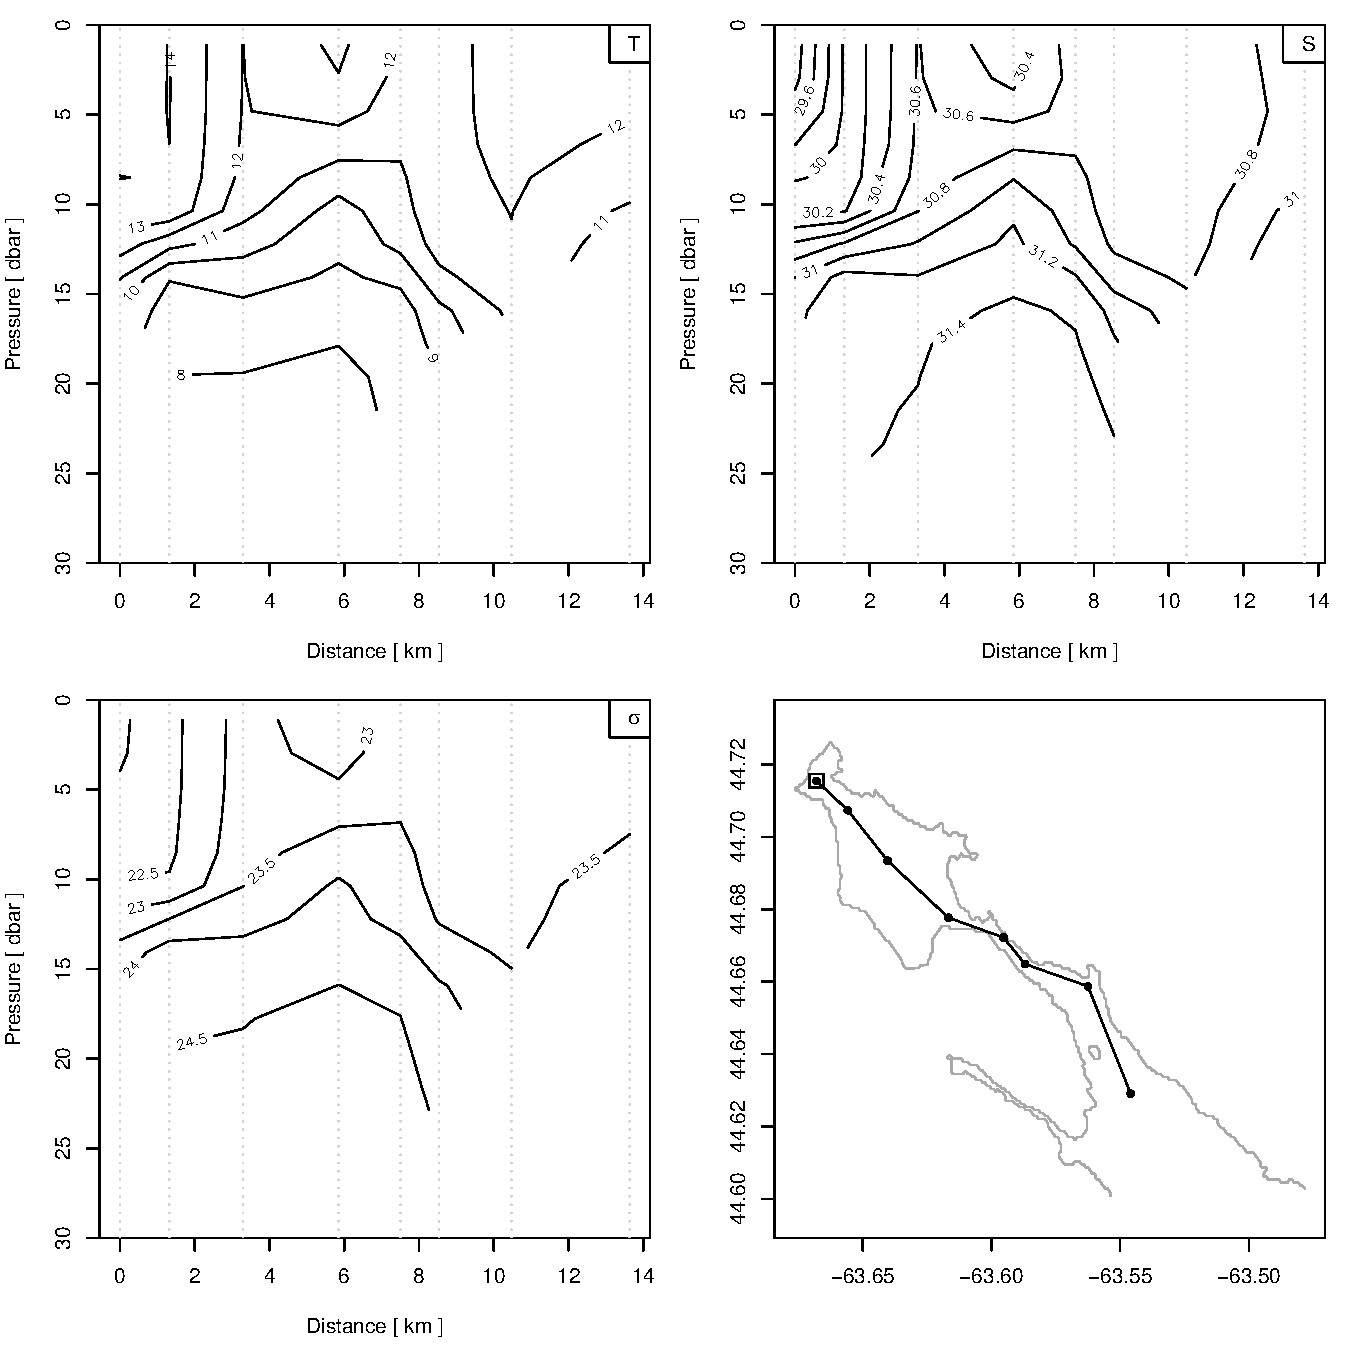
\includegraphics{oce-sectionfig}
\end{center}
\caption{CTD section of data acquired in Halifax Harbour in the autumn of 2003
by students in the \emph{Introduction to Physical Oceanography} class at
Dalhousie University.  (Dan Kelley
teaches this class, but the work at sea was
supervised by his teaching assistant
Natacha Bernier, who received her PhD from Dalhousie in 2005.)
The stations go from a site near
the Sackville river inflow at the northwest portion of Bedford Basin
to site at the entrance of the harbour.}
\label{fig:section}
\end{figure}



\section{Coastline data}
The commands
\begin{Schunk}
\begin{Sinput}
> library(oce)
> data(coastline.maritimes)
> plot(coastline.maritimes, col = "darkred")
> points(-(63 + 34/60), 44 + 39/60, cex = 3, col = "blue")
\end{Sinput}
\end{Schunk}
produce a map of the coastline of Eastern Canada (Figure~\ref{fig:coastline}). Such coastline
data are available from a variety of sources. The NOAA site
\url{http://www.ngdc.noaa.gov/mgg_coastline/}
is particularly popular, and it has the advantage
of providing data in Splus format.
\begin{figure}
\begin{center}
\setkeys{Gin}{width=0.5\textwidth}
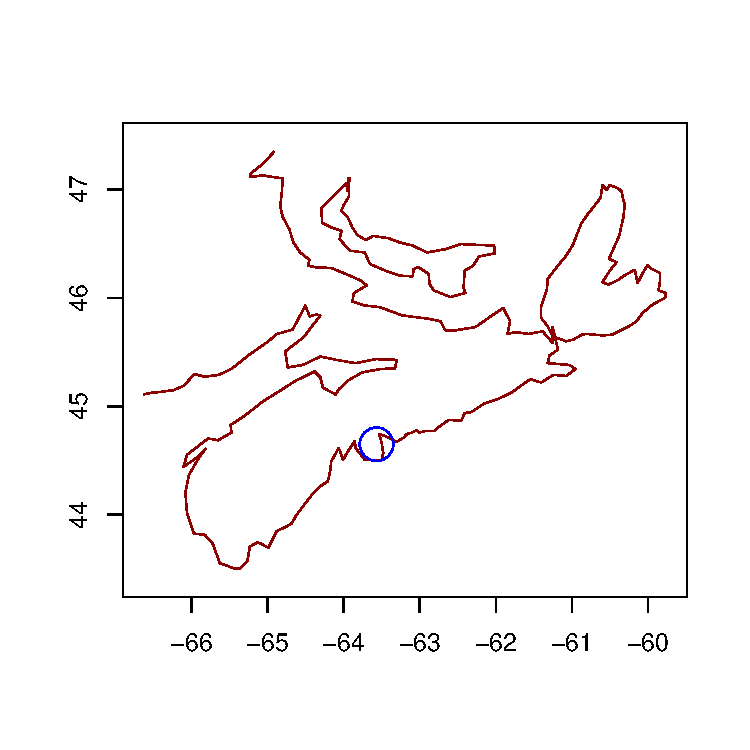
\includegraphics{oce-coastlinefig}
\end{center}
\caption{Coastline of eastern Canada, showing Prince Edward Island, New Brunswick, and Nova Scotia.  The blue circle indicates the location of 
Halifax, the capital of Nova Scotia.}
\label{fig:coastline}
\end{figure}

\section{Sea-level data}

The commands
\begin{Schunk}
\begin{Sinput}
> library(oce)
> data(sealevel)
> plot(sealevel)
\end{Sinput}
\end{Schunk}
load and graph a build-in dataset of sea-level timeseries. The result, shown in
Figure~\ref{fig:sealevel}, is a four-panel plot. The top panel is a timeseries view that
provides an overview of the entire data set. The second panel is narrowed to the most recent
month, which should reveal spring-neap cycles if the tide is mixed. The third panel is a
spectrum, with a few tidal constituents indicated. At the bottom is a cumulative spectrum,
which makes these narrow-banded constituents quite visible.

\begin{figure}
\begin{center}
\setkeys{Gin}{width=.95\textwidth}
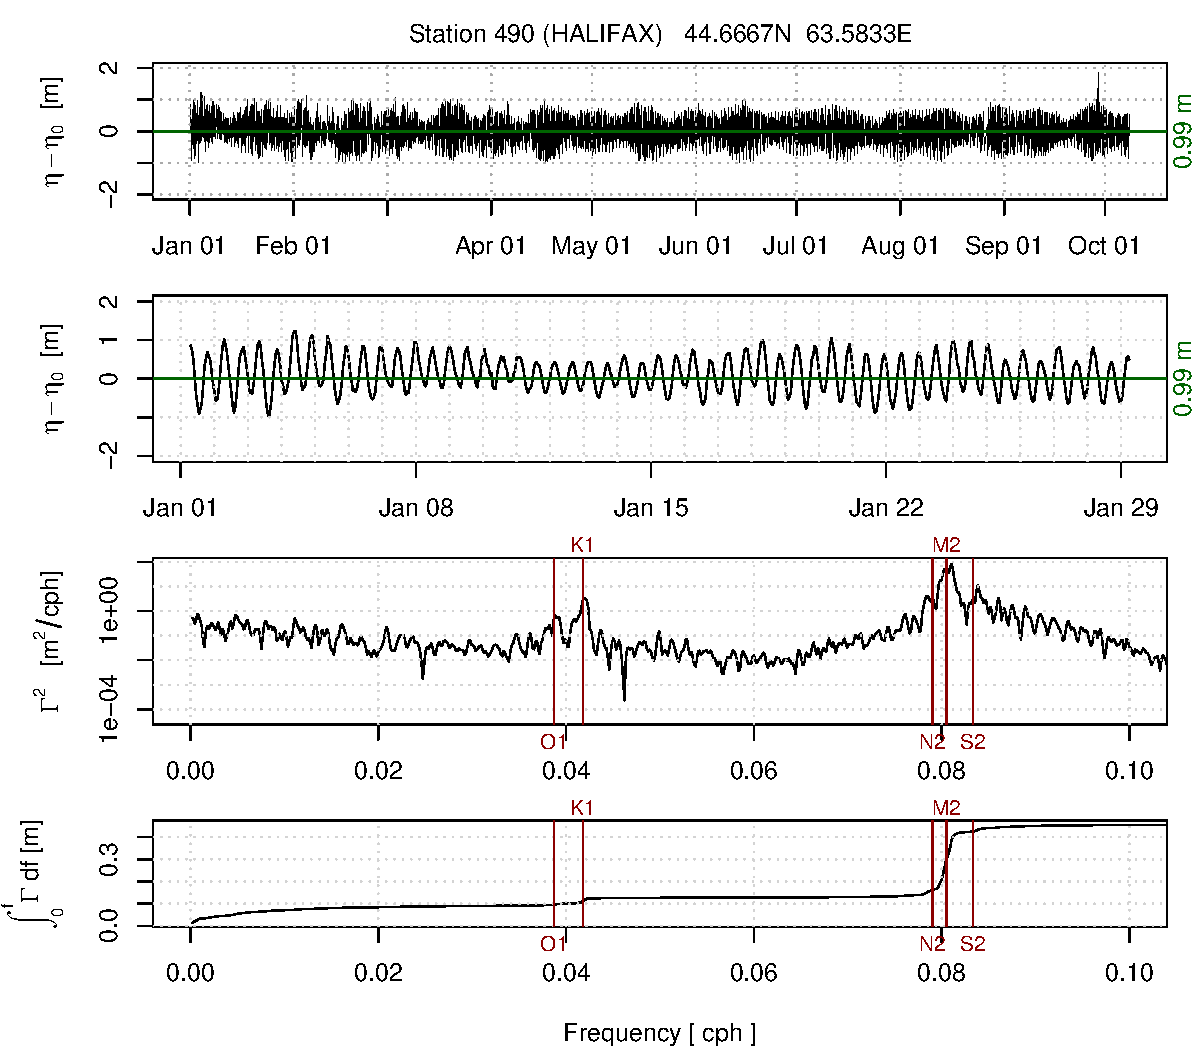
\includegraphics{oce-sealevelfig}
\end{center}
\caption{Sea-level timeseries measured in 2003 in Halifax Harbour.
(The spike in September is the storm
surge associated with Hurricane Juan,
regarded by the Canadian Hurricane Centre to be 
one of the most powerful and damaging
hurricanes to ever hit Canada.}
\label{fig:sealevel}
\end{figure}

\workedexercise{3}{Focus on the spike in sealevel that was caused by Hurricane Juan.}

Note: An upcoming version of \verb@oce@ will also provide tidal constituent analysis. Some of
this has been developed already. The regression works, so that the amplitudes and phases can be
calculated. However, significance levels are not yet provided, and nor is any indication of the
Rayleigh separation of the constituents. The interface also needs work, e.g. for shallow-water
and deep-water cases. If you understand these things, and would like to test the code as it is
being developed, please contact the author. Otherwise, you should wait until the code is
working properly, and until the user interface has settled into a firmer state.

\workedexercise{4}{Draw a spectrum of sealevel variation, with the M2 tidal component indicated.}


\goodbreak

\section{Lobo data}
The commands
\begin{Schunk}
\begin{Sinput}
> library(oce)
> data(lobo)
> plot(lobo)
\end{Sinput}
\end{Schunk}
produce a plot (Figure~\ref{fig:lobo}) of lobo data from the Northwest Arm of Halifax Harbour.
Note the relationship between decreasing nutrients and increasing fluorescence, as well as the
diurnal signal in the latter.  

As an aside, it should be pointed out that the \verb@lobo@ part of \verb@oce@ is somewhat
preliminary. In particular, the package requires that certain data columns be present, and in a
certain order. Also, the function \verb@read.oce@ does not understand \verb@lobo@ files. Why
these limitations, you ask? Well, the \verb@lobo@ code was really only written as an aside, for
the author's contribution to a ``predict the spring bloom'' contest held at Dalhousie
University.

\begin{figure}
\begin{center}
\setkeys{Gin}{width=\textwidth}
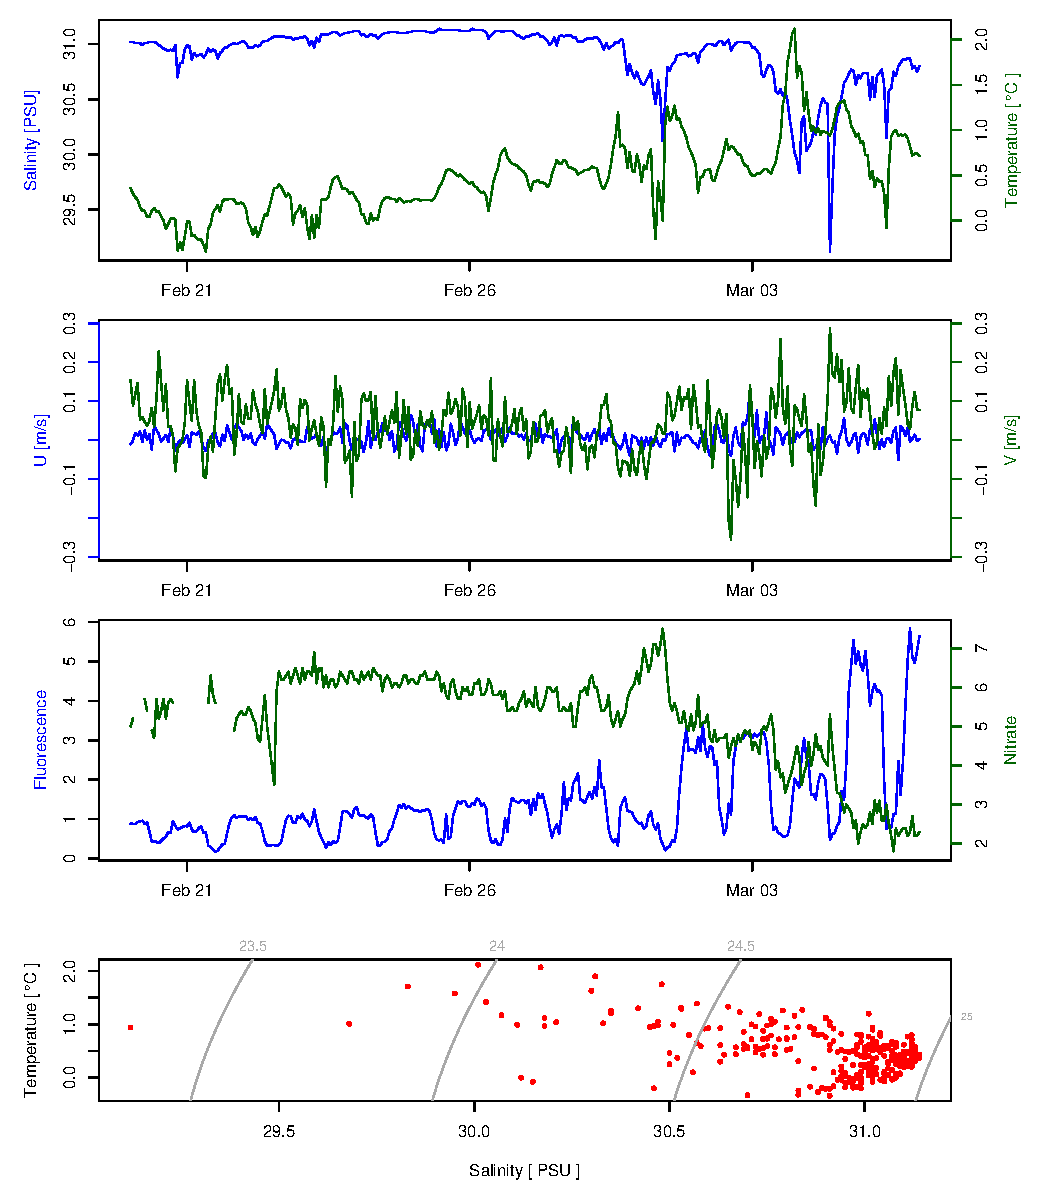
\includegraphics{oce-lobofig}
\end{center}
\caption{Lobo measurements in Northwest Arm of Halifax Harbour, at
the time of the 2007 Spring bloom.}
\label{fig:lobo}
\end{figure}

\workedexercise{5}{Draw a $T-S$ plot for these data, using a colour coding to indicate time,
and using plotting tricks to reduce the obscuring of this time signal.}


\section{The future of oce}

The present version of \verb@oce@ can only handle data types that I have been using lately in my
research. I am quite aware that there are some prominent gaps in the coverage. For example, the
package should handle acoustic-Doppler current profiler data, which are a part of many field
programs. I would like to see \verb@oce@ handle microstructure data as well, but I realize that this
is mostly a personal interest; the wider community probably regards ADCP support as a higher
priority.

Omissions in the category of oceanographic algorithms include tidal analysis, formulae for air-sea
fluxes, and the handling of numerical model output. Tidal analysis will be added soon, but there are
no definite plans for other algorithms, partly because it is not clear which has the highest
priority.

I would like to learn what ideas \verb@oce@ users have for new features. I cannot promise to add
every feature that might be suggested, but I do hope to build up a prioritized list that will
motivate me to apply my time and skill in a useful way.

My hope is that \verb@oce@ will develop into a tool that many oceanographers find to be useful. For
this reason, I hope \verb@oce@ users will take the time to send me reports of bugs, and ideas for
adjustment of existing features, as well as ideas for new features.

\begin{center}

\vspace{2cm}

------

\vspace{2cm}

See the last page of this document for answers to exercises.

\end{center}



\newpage	
	
\section*{Answers to exercises}

\workedanswer{1}
The first two lines should be self-explanatory.  Comparing the last two lines
reveals that \verb@sw.theta@ has an optional parameter \verb@pref@ that gives 
the reference pressure.  Consult the documentation (e.g. \verb@?sw.rho@) for the 
details of these parameters.
\begin{Schunk}
\begin{Sinput}
> sw.rho(S = 34, t = 10, p = 100)
> sw.theta(S = 34, t = 10, p = 100)
> sw.rho(S = 34, t = sw.theta(S = 34, t = 10, p = 100), p = 0)
> sw.rho(S = 34, t = sw.theta(S = 34, t = 10, p = 100, pref = 200), 
+     p = 200)
\end{Sinput}
\end{Schunk}

\workedanswer{2}
One may argue as to the limits of the pycnocline, taken for illustration here to be the range from 5dbar to 12dbar.
\begin{Schunk}
\begin{Sinput}
> library(oce)
> data(ctd)
> pycnocline <- ctd.trim(ctd, "pressure", c(5, 12))
> plot.profile(pycnocline, type = "sigmatheta+N2")
\end{Sinput}
\end{Schunk}

\workedanswer{3} A web search will tell you that Hurricane Juan hit about midnight, 2003-sep-28.
The author can verify that the strongest winds occurred a bit after midnight -- that was the time
he moved to a room without windows to escape from the threat of flying glass.
\begin{Schunk}
\begin{Sinput}
> library(oce)
> data(sealevel)
> plot(sealevel, focus.time = c("2003-09-23", "2003-10-05"))
> abline(v = as.POSIXct("2003-09-28 23:30:00"), col = "red", lty = "dotted")
> mtext("Hurricane\nJuan", at = as.POSIXct("2003-09-28 23:30:00"), 
+     col = "red")
\end{Sinput}
\end{Schunk}

\workedanswer{4}
Notice the use of \verb@(object)$data$(item)@ here.  All \verb@oce@ objects are lists, 
and all of them contain a \verb@data@ element of a similar form to this.
\begin{Schunk}
\begin{Sinput}
> library(oce)
> data(sealevel)
> spectrum(sealevel$data$eta, spans = c(3, 7))
> abline(v = 1/12.42)
> mtext("M2", at = 1/12.42, side = 3)
\end{Sinput}
\end{Schunk}

\workedanswer{5}
The resampling with \verb@i@ is to avoid obscuring colours by overplotting.  Note 
the use of \verb@as.CTD@ to assemble the data into something that \verb@plot.TS@ can handle.
This is an example of the practicality of \verb@oce@; eventually, \verb@plot.TS@ may be altered to take simple columns of data, but for now it seems reasonable to require the user to assemble
these data into a CTD object, and to spend development time on something that will pay
off better.
\begin{Schunk}
\begin{Sinput}
> library(oce)
> data(lobo)
> i <- sample(length(lobo$T))
> a <- as.numeric(lobo$time[i] - lobo$time[1])
> col <- hsv(0.5 * a/max(a), 1, 1)
> plot.TS(as.CTD(lobo$S[i], lobo$T[i], 0), col = col, pch = 1)
\end{Sinput}
\end{Schunk}

\end{document}

